%%%%%%%%%%%%%%%%%%%%%%%%%%%%%%%%%%%%%%%%%
% Masters/Doctoral Thesis 
% LaTeX Template
% Version 1.43 (17/5/14)
%
% This template has been downloaded from:
% http://www.LaTeXTemplates.com
%
% Original authors:
% Steven Gunn 
% http://users.ecs.soton.ac.uk/srg/softwaretools/document/templates/
% and
% Sunil Patel
% http://www.sunilpatel.co.uk/thesis-template/
%
% License:
% CC BY-NC-SA 3.0 (http://creativecommons.org/licenses/by-nc-sa/3.0/)
%
% Note:
% Make sure to edit document variables in the Thesis.cls file
%
%%%%%%%%%%%%%%%%%%%%%%%%%%%%%%%%%%%%%%%%%

%----------------------------------------------------------------------------------------
%	PACKAGES AND OTHER DOCUMENT CONFIGURATIONS
%----------------------------------------------------------------------------------------

\documentclass[11pt, oneside]{Thesis} % The default font size and one-sided printing (no margin offsets)

\graphicspath{{Images/}{Charts/}} % Specifies the directory where pictures are stored
\usepackage{times}
\usepackage{pdfpages}
\usepackage{subfigure}
\usepackage[square, numbers, comma, sort&compress]{natbib} % Use the natbib reference package - read up on this to edit the reference style; if you want text (e.g. Smith et al., 2012) for the in-text references (instead of numbers), remove 'numbers' 
\usepackage{amsmath}
\usepackage{amssymb}
\usepackage{graphicx}
\usepackage{listings}
\usepackage{siunitx}
\usepackage{float}
% For algorithms management
\usepackage[linesnumbered, ruled]{algorithm2e}
\SetKwRepeat{Do}{do}{while}%

\lstset{
	language=C++,
	basicstyle=\ttfamily,
	keywordstyle=\color{blue}\ttfamily,
	stringstyle=\color{red}\ttfamily,
	commentstyle=\color{teal}\ttfamily,
	columns=flexible,
	}

\hypersetup{urlcolor=blue, colorlinks=true} % Colors hyperlinks in blue - change to black if annoying
\title{\ttitle} % Defines the thesis title - don't touch this

\begin{document}
\frontmatter % Use roman page numbering style (i, ii, iii, iv...) for the pre-content pages

\setstretch{1.3} % Line spacing of 1.3

% Define the page headers using the FancyHdr package and set up for one-sided printing
\fancyhead{} % Clears all page headers and footers
\rhead{\thepage} % Sets the right side header to show the page number
\lhead{} % Clears the left side page header

\pagestyle{fancy} % Finally, use the "fancy" page style to implement the FancyHdr headers

\newcommand{\HRule}{\rule{\linewidth}{0.5mm}} % New command to make the lines in the title page
\newcommand{\datasetunimore} {Interactive Museum}
\newcommand{\argmax}{\arg\!\max}
% PDF meta-data
\hypersetup{pdftitle={\ttitle}}
\hypersetup{pdfsubject=\subjectname}
\hypersetup{pdfauthor=\authornames}
\hypersetup{pdfkeywords=\keywordnames}

%----------------------------------------------------------------------------------------
%	TITLE PAGE
%----------------------------------------------------------------------------------------

\begin{titlepage}

\begin{center}
\textsc{\Large \bf \univname}\\[0.5cm] % University name
\textsc{\large Dipartimento di Ingegneria ``Enzo Ferrari"}\\[0.2cm] % Thesis type
%\HRule \\ % Horizontal line
\textsc{\large Corso di Laurea Magistrale in Ingegneria Informatica}\\[5.0cm] % Thesis type

\HRule \\[0.6cm] % Horizontal line
{\huge \bfseries \ttitle}\\[0.4cm] % Thesis title
%\HRule \\[0.6cm] % Horizontal line
%{\huge \bfseries \ttitleITA}\\[0.4cm] % Thesis title
\HRule \\[3.2 cm] % Horizontal line
 
\begin{minipage}{0.4\textwidth}
\begin{flushleft} \large
\emph{Candidato:}\\
\authornames % Author name - remove the \href bracket to remove the link
\end{flushleft}
\end{minipage}
\begin{minipage}{0.4\textwidth}
\begin{flushright} \large
\emph{Relatore:} \\
\supname \\ % Supervisor name - remove the \href bracket to remove the link  
\emph{Correlatore:} \\
\cosupname \\ % Supervisor name - remove the \href bracket to remove the link  
\end{flushright}
\end{minipage}\\[5.0cm]
 
%\large \textit{A thesis submitted in fulfilment of the requirements\\ for the degree of \degreename}\\[0.3cm] % University requirement text
%\textit{in the}\\[0.4cm]
%\groupname\\\deptname\\[2cm] % Research group name and department name
 
\textsc{\large Anno Accademico 2021-2022}\\[4cm] % Date
%\includegraphics{Logo} % University/department logo - uncomment to place it
 
\vfill
\end{center}

\end{titlepage}

\clearpage % Start a new page

%----------------------------------------------------------------------------------------
%	SYMBOLS
%----------------------------------------------------------------------------------------

%\clearpage % Start a new page
%
%\lhead{\emph{Symbols}} % Set the left side page header to "Symbols"
%
%\listofnomenclature{lll} % Include a list of Symbols (a three column table)
%{
%$a$ & distance & m \\
%$P$ & power & W (Js$^{-1}$) \\
%% Symbol & Name & Unit \\
%
%& & \\ % Gap to separate the Roman symbols from the Greek
%
%$\omega$ & angular frequency & rads$^{-1}$ \\
%% Symbol & Name & Unit \\
%}
\newcommand{\etal}{\textit{et al.~}}

%----------------------------------------------------------------------------------------
%	ABSTRACT PAGES
%----------------------------------------------------------------------------------------
\addtotoc{Abstract in English} % Add the "Abstract" page entry to the Contents
%
\englishAbstract{\addtocontents{toc}{\vspace{1em}} % Add a gap in the Contents, for aesthetics

\textbf{Keywords:} Medical Imaging, Cone Bean Computed Tomography, Inferior Alveolar Canal, Image Segmentation, Deep Learning.
}
\clearpage % Start a new page

\addtotoc{Abstract in Italian} % Add the "Abstract" page entry to the Contents
\italianAbstract{\addtocontents{toc}{\vspace{1em}} % Add a gap in the Contents, for aesthetics

\textbf{Parole Chiave:} Medical Imaging, Cone Bean Computed Tomography, Inferior Alveolar Canal, Image Segmentation, Deep Learning.
}
\clearpage % Start a new page

%----------------------------------------------------------------------------------------
%	SINTESI IN ITALIANO PAGES
%----------------------------------------------------------------------------------------

\addtotoc{Summary in Italian} % Add the "Abstract" page entry to the Contents
%
\italianSummary{\addtocontents{toc}{\vspace{1em}} % Add a gap in the Contents, for aesthetics
%
Il regolamento della Facoltà di Ingegneria di Modena prevede che le tesi scritte
in lingua inglese debbano contenere un \textit{abstract} ed un'ampia sintesi dei
contenuti in lingua italiana: in accordo a questa regola, proponiamo un sunto
degli argomenti, delle tecniche e dei risultati che verranno delineati
nell'elaborato. Si noti che non si tratta di un sunto esaustivo, e che non è
possibile valutare la tesi dalla semplice lettura di queste righe. Per una
descrizione più dettagliata e più rigorosa, e per i risultati sperimentali
ottenuti, si rimanda al testo in inglese.

Questa tesi tratta del... Durante il lavoro svolto è inoltre stato pubblicato un
\textit{paper} attualmente in fase di revisione (si veda l’Appendice per
ulteriori dettagli).

}
%
\clearpage % Start a new page

%----------------------------------------------------------------------------------------
%	DEDICATION
%----------------------------------------------------------------------------------------
\mainmatter
\setstretch{1.3} % Return the line spacing back to 1.3

\pagestyle{empty} % Page style needs to be empty for this page

\dedicatory{To ...} % Dedication text

\addtocontents{toc}{\vspace{2em}} % Add a gap in the Contents, for aesthetics

%----------------------------------------------------------------------------------------
%	ACKNOWLEDGEMENTS
%----------------------------------------------------------------------------------------

\setstretch{1.3} % Reset the line-spacing to 1.3 for body text (if it has changed)

\acknowledgements{\addtocontents{toc}{\vspace{1em}} % Add a gap in the Contents, for aesthetics

Foremost, I would like to express my sincere gratitude to ...
}
\clearpage % Start a new page

%----------------------------------------------------------------------------------------
%	LIST OF CONTENTS/FIGURES/TABLES PAGES
%----------------------------------------------------------------------------------------

\pagestyle{fancy} % The page style headers have been "empty" all this time, now use the "fancy" headers as defined before to bring them back

\lhead{\emph{Contents}} % Set the left side page header to "Contents"
\tableofcontents % Write out the Table of Contents

\lhead{\emph{List of Figures}} % Set the left side page header to "List of Figures"
\listoffigures % Write out the List of Figures

\lhead{\emph{List of Tables}} % Set the left side page header to "List of Tables"
\listoftables % Write out the List of Tables

\lhead{\emph{List of Listings}} % Set the left side page header to "List of Listings"
\lstlistoflistings % Write out the List of Listings

%----------------------------------------------------------------------------------------
%	ABBREVIATIONS
%----------------------------------------------------------------------------------------

%\clearpage % Start a new page
%
%\setstretch{1.5} % Set the line spacing to 1.5, this makes the following tables easier to read
%
%\lhead{\emph{Abbreviations}} % Set the left side page header to "Abbreviations"
%\listofsymbols{ll} % Include a list of Abbreviations (a table of two columns)
%{
%\textbf{LAH} & \textbf{L}ist \textbf{A}bbreviations \textbf{H}ere \\
%%\textbf{Acronym} & \textbf{W}hat (it) \textbf{S}tands \textbf{F}or \\
%}

%----------------------------------------------------------------------------------------
%	PHYSICAL CONSTANTS/OTHER DEFINITIONS
%----------------------------------------------------------------------------------------

%\clearpage % Start a new page
%
%\lhead{\emph{Physical Constants}} % Set the left side page header to "Physical Constants"
%
%\listofconstants{lrcl} % Include a list of Physical Constants (a four column table)
%{
%Speed of Light & $c$ & $=$ & $2.997\ 924\ 58\times10^{8}\ \mbox{ms}^{-\mbox{s}}$ (exact)\\
%% Constant Name & Symbol & = & Constant Value (with units) \\
%}


%----------------------------------------------------------------------------------------
%	THESIS CONTENT - CHAPTERS
%----------------------------------------------------------------------------------------

 % Begin numeric (1,2,3...) page numbering

\pagestyle{fancy} % Return the page headers back to the "fancy" style

% Include the chapters of the thesis as separate files from the Chapters folder
% Uncomment the lines as you write the chapters

% Chapter 1

\chapter{Segmentation of the Inferior Alveolar Canal: an overview}

\lhead{Chapter 1. \emph{Segmentation of the Inferior Alveolar Canal}} % This is for the header on each page - perhaps a shortened title
\label{chp:introductive_chapter}
%----------------------------------------------------------------------------------------

\def\:{\hskip0pt} %Definisce un modo veloce per permettere a latex di sillabare correttamente anche parole come 4-connectivity. Il corretto utilizzo è il seguente: 4\:-\:connectivity.

\section{Introduction}
Dental implant placement within the jawbone is a routine surgical procedure that
can become complicated due to the presence of the Inferior Alveolar Nerve (IAN)
nearby. The nerve, in particular, is frequently in close proximity to the roots
of molars, and its position must thus be meticulously detailed prior to surgical
removal. Avoiding contact with the IAN is a primary concern during these
operations, thus its segmentation is crucial in surgical planning.
Today the standard de-facto is to take a CBCT scan of the jawbone and a 2D
panomaric view is extracted. This view allow medical experts to depict the IANs
position with line. We refer to this type of annotation as \emph{sparse} or
\emph{2D} annotation. A 3D annotation of the IAC is often avoided as it would
require a huge amount of time, but this type of segmentation would offer a much
precise knowledge of the position of the IAN and IAC and could allow dentists to
plan a more detailed surgical approach. For this reason a lot of research about
automatic segmentation of the IAC has been carried out and is still active today.\\

In this chapter we first describe in details the role of the IAN and the IAC,
what a CBCT is and the definitions and carachteristics of different types of
segmentations.
In the following chapter we will take a look on how segmentation is performed
today using neural networks paying more attention field of medical images.
Next in chapter 3 we will detail the dataset, the network, the metrics, and
other tools used as baseline to define the current state of the art, which is
essential to understand the importance and goodness of the work that i've
carried out. Last, in chapter 4, all the different techniques tried will be
described in details, to conclude with a description of which would possible be
the future work for this specific tasks.

\section{Inferior Alveolar Canal}
The Inferior Alveolar Canal (IAC) is a small passageway shaped as a tube that
runs through the lower jawbone. It houses the Inferior Alveolar Nerve (IAN),
which is responsible for transmitting sensory information from the teeth, gums
and lips to the brain. It also provides motor innervation to the muscles of
mastication (i.e. the muscles responsible for chewing). Dentists need to be able
to accurately locate the IAC before performing certain surgical operations, such
as tooth extractions or placement of dental implants. This is because the IAC is
located very close to the roots of the teeth, and damage to the IAC during
surgery can result in permanent nerve damage which would cause numbness,
tingling, and pain in the affected area. In severe cases, it can also lead to
muscle weakness and paralysis.

\section{Cone Beam Computed Tomography}
Cone beam computed tomography (CBCT) is a medical imaging technique consisting
of X-ray computed tomography where rays are divergent, forming a cone. This type
of computed tomography is well suited for imaging the craniofacial area as it
provides clear images of highly contrasted structures, very helpfull to
evaluate bones. It has become common in dentistry such as oral surgery,
endodontics and orthodontics.
The main reasons and advantages of CBCT with respect to other CTs are:
\begin{enumerate}
  \item{\textbf{X-ray beam limitation:} reducing the size of the irradiated area
  by collimating the primary x-ray beam to the are of interest minimizes the
  radiation dose. Most CBCT units can be adjusted to scan small regions for
  specific diagnostic task. They are also able to scan the whole craniofacial
  structure if needed.}
  \item{\textbf{Image accuracy:} We created a novel, large, and publicly
  available maxillo-facial CBCT (Cone Beam Computed Tomography) dataset, with 2D
  and 3D manual annotations, provided by expert clinicians. All CBCT units
  provide voxel resolutions that are isotropic (i.e. equals in all the 3
  dimensions) while in conventional CT, voxel are anisotripic (i.e. rectangular
  cubes).}
  \item{\textbf{Rapid scan time:} CBCT acquires all the basis images in a single
  rotation, thus scan time goes from 10s to 70s. Although faster scanning time
  usually means fewer basis images from which to reconstruct the volumetric
  dataset, motion artifacts due to subject movement are reduced.}
\end{enumerate}
These advantages come with some drawbacks: Hounsfield units (HU) is the metric
used to determine the radiodensity of tissue analized. In the Hounsfield scale,
numbers go from values of $-1000$ for air to values of $1600$ for dense bones.
In CBCT scans, the radiodensity is inaccurate because different areas in the
scan appear with different greyscale values depending on their relative
positions in the organ being scanned, despite possessing identical densities,
because the image value of a voxel of an organ depends on the position in the
image volume. HU measured from the same anatomical area with both CBCT and
medical-grade CT scanners are not identical and are thus unreliable for
determination of site-specific, radiographically-identified bone density for
purposes such as the placement of dental implants, as there is "no good data to
relate the CBCT HU values to bone quality" \cite{Miles2007}.\\
The images resulting from a CBCT scans are usually exported as DICOM (Digital
Imaging and Communications in Medicine) which is the standard used worldwide to
store, exchange, and transmit medical images.

\section{DICOM file format}
TODO?

\section{Image Segmentation}
Image segmentation is a well known topic in computer and image processing with a
wide range of application, such as medical imaging, robotics, video
surveillance, etc.
It involves partitioning images into one or more objects and can also includes
classify these objects. Many traditional algorithms have been developed in the
literature but, in the most recent years, they have all been dominated by deep
neural networks. Since the 2015 a huge amount of different types of networks
that aim to perform image segmentation has been proposed for each of the field
where it's needed.
Before presenting how nowday segmentation is performed, we must state which are
the different type of segmentation that have been classified:

\begin{itemize}
  \item{\textbf{Semantic segmentation:}
  Semantic Segmentation perform a pixel-by-pixel classification with a predefined
  set of objects categories for all the pixels of the images. In pratice, given a
  RGB image (\texttt{height} $\times$ \texttt{width} $\times$ \texttt{3}) we output
  a segmentation map of size (\texttt{height} $\times$ \texttt{width} $\times$
  \texttt{classes}) where each value correspond to which class the same pixel in the
  original images belongs.}

  \item{\textbf{Instance segmentation:}
  One possible issue of semantic segmentation is that it doesn't allow to
  distinguish two or more object of the same class when they overlap in the image.
  Instance segmentation overcome this problem by outputting a different number of
  channels based on the number of instances present in the image.}

  \item{\textbf{Panoptic segmentation:}
  The latter type of segmentation is called Panoptic segmentation and is the
  result of the previously presented method joined together. The difference with
  the instance segmentation is that in this case instances are not allowed to
  overlap then for to a single pixel, a single instance must be assigned.}
\end{itemize}

% Figure 1: example of a segmentation on mri image
\begin{figure}[h]
  \centering
  \includegraphics[width=0.8\textwidth]{Images/example_segmentation.png}
  \caption{Example of a multiclass semantic segmentation, different colors represent different classes}
  \label{fig:segmentation}
\end{figure}



% \section{Segmentation using Deep Neural Networks}
% As stated before, nowdays deep learning is the dominant method used for
% segmentation. Convolutional Neural Networks are still the most used type of
% networks used to date but new promising technique, as Graph Neural Networks or
% Transformers, are always more and more used.

% Chapter 2

\chapter{Segmentation Neural Networks}

\lhead{Chapter 2. \emph{Segmentation Neural Networks}} % This is for the header on each page - perhaps a shortened title
\label{chp:cbct}
%----------------------------------------------------------------------------------------

\def\:{\hskip0pt} %Definisce un modo veloce per permettere a latex di sillabare correttamente anche parole come 4-connectivity. Il corretto utilizzo è il seguente: 4\:-\:connectivity.

\section{Segmentation using Deep Neural Networks}
\label{sec:segmentation}
Today, deep neural netoworks are the state-of-the-art in many fields, including
image segmentation. In this section, we will briefly review the most common
approaches to segmentation using deep neural networks, and we will discuss the
advantages and disadvantages of each approach.

\subsection{Fully Convolutional Networks}
\label{sec:fcn}
Fully convolutional networks (FCNs) are a class of deep neural networks that
are designed to perform pixel-wise classification. The main idea behind FCNs is
to use a convolutional neural network (CNN) to extract features from the input
image and return an output of the same size as the input image, where each
pixel is assigned a class label. The main advantage of FCNs is that they can be
trained end-to-end, which means that the network can be trained to perform the
classification of each pixel without the need of any post-processing step. On
the other hand, Deep Neural Networks lacks for explainability, which is a major
drawback for medical applications.
The architecture of such networks can be grouped as shown in Figure \ref{fig:fcn_architecture}.
\begin{figure}[ht]
  \centering
  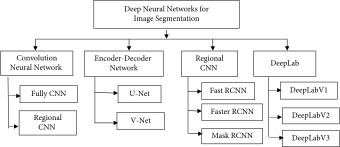
\includegraphics[width=0.8\linewidth]{Images/seg-arch.png}
  \caption{Groups of a segmentation network architecture.}
  \label{fig:fcn_architecture}
\end{figure}

\subsection{Convolutional Neural Networks}
A convolutional neural network or CNN consists of a stack of
three main neural layers: convolutional layer, pooling layer, and fully
connected layer. Each layer has its own role. The convolution layer
detects distinct features like edges or other visual elements in an image.
Convolution layer performs mathematical operation of multiplication of local
neighbours of an image pixel with kernels. CNN uses different kernels for
convolving the given image for generating its feature maps. Pooling layer
reduces the spatial \texttt{(width, height)} dimensions of the input data for the next
layers of neural network. It does not change the depth of the data. This
operation is called as subsampling. This size reduction decreases the
computational requirements for upcoming layers. The fully connected layers
perform high-level reasoning in NN. These layers integrate the various feature
responses from the given input image so as to provide the final results.\\
Different CNN models have been reported in the literature, including AlexNet,
GoogleNet, VGG, Inception, SequeezeNet, and DenseNet. This type of networks were
mostly used for classification, but they have been easily adapted to perform
segmentation.

\subsection{Fully Convolutional Networks}
In fully convolutional network (FCN), only convolutional layers exist. The
different existing in CNN architectures can be modified into FCN by converting
the last fully connected layer of CNN into a fully convolutional layer. This
type of networks can output spatial segmentation map and can have dense
pixel-wise prediction from the input image of full size instead of performing
patch-wise predictions. They can also uses skip connections, when performing upsampling
on feature maps from final layer, these skip connections fuses it with the
feature map of previous layers. The model thus produces a detailed segmentation
in just one go but as drawback they do not have a global context of the image
and the output can be fuzzy close to the boundaries of segmented objects.

\subsection{Encoder-Decoder Networks}
Encoder-decoder based models employ two-stage model to map data points from the
input domain to the output domain. The encoder stage compresses the given input
to a latent space representation, while the decoder predicts the output from
this representation. This latent space representation is a compressed version of
the input image, which is used to generate the output, it have smaller spatial dimension
than the input image but an increased depth. In order to upsample this latent space representation
to the size of the input image, transposed convolutional layers are used.
One of the most popular encoder-decoder networks is the U-Net
\cite{ronneberger2015u}, for which we can find in literature many variants. The
U-Net architecture is shown in Figure \ref{fig:unet_architecture}.
% \begin{figure}[ht]
%   \centering
  % \includegraphics[width=0.8\linewidth]{Images/unet-arch.png}
  % \caption{U-Net architecture.}
  % \label{fig:unet_architecture}
% \end{figure}
U-Net model has a downsampling and upsampling part. The downsampling
section with FCN like architecture extracts features using $3 \times 3$ convolutions to
capture context. The upsampling part performs deconvolution to decrease the
number of computed feature maps. The feature maps generated by downsampling or
contracting part are fed as input to upsampling part so as to avoid any loss of
information. The symmetric upsampling part provides precise localization. The
model generates a segmentation map which categorizes each pixel present in the
image. This type of architecture proposed in 2015 is still widely used today as
it can obtain state-of-the-art resuts.

\subsection{Regional Convolutional Neural Networks}
Regional convolutional network has been utilized for object detection and
segmentation task. The R-CNN architecture presented in [69] generates region
proposal network for bounding boxes using selective search process. These region
proposals are then warped to standard squares and are forwarded to a CNN so as
to generate feature vector map as output. The output dense layer consists of
features extracted from the image and these features are then fed to
classification algorithm so as to classify the objects lying within the region
proposal network. The algorithm also predicts the offset values for increasing
the precision level of the region proposal or bounding box. The processes
performed in R-CNN architecture are shown in Figure 4. The use of basic RCN
model is restricted due to the following:

\subsection{DeepLab}
DeepLab model employs pretrained CNN model ResNet-101/VGG-16 with atrous
convolution to extract the features from an image. The use of atrous
convolutions gives the following benefits:
\begin{itemize}
  \item{It controls the resolution of feature responses in CNNs}
  \item{It converts image classification network into a dense feature extractor
    without the requirement of learning of any more parameters employs
    conditional random field (CRF) to produce fine segmented output}
\end{itemize}
The various variants of DeepLab have been proposed in the literature including
DeepLabv1, DeepLabv2, DeepLabv3, and DeepLabv3+.
In DeepLabv1, the input image is passed through deep CNN layer with one or
two atrous convolution layers. This generates a coarse feature map. The feature
map is then upsampled to the size of original image by using bilinear
interpolation process. The interpolated data is applied to fully connect
conditional random field to obtain the final segmented image.

\section{Dealing with 3D Medical Images}
It is not uncommon in the medical field to deal with 3D images that comes from
CT scans or MRI scans. In this case, a 3D image can be represented as a stack of
2D images and fed them to the network. Each output is then stacked back to
produce the final 3D output. Another approach is to use 3D convolutional
networks. The 3D convolutional network is a generalization of the 2D
convolutional network to 3D data.
In the first case, each 2D layer is indipendend from the others, while in the
second case, the 3D convolutional network is able to learn the spatial
relationships between the different slices of the 3D image.


% % Chapter 3

\chapter{Image Segmentation}

\lhead{Chapter 3. \emph{Image Segmentation}} % This is for the header on each page - perhaps a shortened title
\label{chp:segmentation}
%----------------------------------------------------------------------------------------

\def\:{\hskip0pt} %Definisce un modo veloce per permettere a latex di sillabare correttamente anche parole come 4-connectivity. Il corretto utilizzo è il seguente: 4\:-\:connectivity.

\section{Introduction}
Image segmentation is a well known topic in computer and image processing with a
wide range of application, such as medical imaging, robotics, video
surveillance, etc.
It involves partitioning images into one or more objects and can also includes
classify these objects. Many traditional algorithms have been developed in the
literature but, in the most recent years, they have all been dominated by deep
neural networks. Since the 2015 a huge amount of different types of networks
that aim to perform image segmentation has been proposed for each of the field
where it's needed.
Before presenting how nowday segmentation is performed, we must state which are
the different type of segmentation that have been classified.

\subsection{Semantic Segmentation}
Semantic Segmentation perform a pixel-by-pixel classification with a predefined
set of objects categories for all the pixels of the images. In pratice, given a
RGB image (\texttt{height} $\times$ \texttt{width} $times$ \texttt{3}) we output
a segmentation map of size (\texttt{height} $\times$ \texttt{width} $\times$
\texttt{1}) where each value correspond to which class the same pixel in the
original images belongs.

\subsection{Instance segmentation}
One possible issue of semantic segmentation is that it doesn't allow to
distinguish two or more object of the same class when they overlap in the image.
Instance segmentation overcome this problem by outputting a different number of
channels based on the number of instances present in the image.

\subsection{Panoptic segmentation}
The latter type of segmentation is called Panoptic segmentation and is the
result of the previously presented method joined together. The difference with
the instance segmentation is that in this case instances are not allowed to
overlap then for to a single pixel, a single instance must be assigned.

\subsection{Segmentation using Deep Neural Networks}
As stated before, nowdays deep learning is the dominant method used for
segmentation. Convolutional Neural Networks are still the most used type of
networks used to date but new promising technique, as Graph Neural Networks or
Transformers, are always more and more used.

% % Chapter 4

\chapter{Code Refactoring}

\lhead{Chapter 4. \emph{Code Refactoring}} % This is for the header on each page - perhaps a shortened title
\label{chp:refwork}
%----------------------------------------------------------------------------------------

\def\:{\hskip0pt} %Definisce un modo veloce per permettere a latex di sillabare correttamente anche parole come 4-connectivity. Il corretto utilizzo è il seguente: 4\:-\:connectivity.
\section{Introduction}
Cipriano et al. spent some effort developing the dataset and a to design a
network which was capable to perform the segmentation of the Inferior Alveolar
Canal.
Together with the novel dataset, they proposed a modified version of
U-Net 3D as a backbone for both the label propagation and the IAC segmentation.
Both these networks and methods were introduced in the previous
chapters and will be explained more in detail in the following sections.
As the code was written near the deadline for the submission of the paper,
the authors did not have focused on producing a codebase that was optimized for
reusability, extensibility, and efficiency.
For this reason, my work starts by refactoring the codebase to add these features
which improved all my successive experiments.

\section{Reference Work}
The reference work that has been taken as starting point for this work has been
made by Cipriano et al. in 2022 \cite{cipriano2022improving}.
The pipeline proposed can be divided into two main steps: the deep label
propagation and the IAC segmentation.

\subsection{Positional PadUNet3D}
A slightly modified version of 3D U-Net has been proposed as a backbone for both
steps. Differently from the original 3D U-Net architecture, every
three-dimensional convolution in our CNN applies 2 pixels padding along each
dimension. Although this alteration does not cause any variation in terms of
performance, it ensures that the output of each convolution has the same size as
its input along axis \emph{x}, \emph{y}, and \emph{z}.

Resolution changes are therefore due uniquely to the three max-pooling layers,
each halving the size of the volumes. When using the aforementioned input size,
the encoder output is composed of $512$ feature maps of size $10 \times 10
\times 10$. Inside the decoder, on the other hand, resolution changes are caused
by transposed convolutions, with dimensions $2 \times 2 \times 2$ for both the
kernel and stride to double the size of the feature maps. This adjustment
ensures resolution symmetry between features in the decoder and corresponding
maps in the encoder, thus allowing them to be simply concatenated with skip
connections. Moreover, the output of the model naturally has the same dimensions
as the input. The final output is a single channel volume, to which we apply a
Sigmoid activation function and a threshold at $0.5$ to obtain the final binary
prediction mask.

The segmentation architecture is further enriched with a positional embedding.
Since our sub-volumes are extracted from the original scan following a fixed
grid, we exploit positional information derived from the location of the
top-left and bottom-right corners of the sub-volume. Specifically, these global
coordinates are fed to a linear layer which yields a single feature map of
dimensions $10 \times 10 \times 10$. This positional embedding gets concatenated
to the output of the encoder, and then fed to the decoder. Exploiting positional
information ensures two extremely important benefits:
\begin{itemize}
  \item{During training, the CNN is fed with implicit information about areas
  close to the edges of the scan, where the IAN is very unlikely to be present.
  This piece of knowledge greatly reduces the number of false positives during
  inference. As a matter of fact, no postprocessing method is required to refine
  the output of the proposed CNN}
  \item{Information about cut positions helps the network to better shape the
  output: sub-volumes located close to the mental foramen generally present a
  much thinner canal than those located in the mandibular foramen. This
  technique could indeed be employed for several classes of medical data, as
  anatomical structures can substantially vary according to their location.}
\end{itemize}

\subsection{Deep Label Propagation}
The presence of a new 3D voxel-level annotated dataset paves the way to a new
frontier for label propagation: we can indeed employ 3D annotations to supervise
a deep label propagation neural network, trained to expand sparse labels into
dense ones, and produce high-quality synthetic ground truths for the
segmentation task. We christen this new label propagation approach Deep Label
Expansion, or Deep Expansion in short. The deep expansion model is based on the
proposed segmentation network, Positional PadUNet. The main difference regards
the input layer, which is changed in order to accept a concatenation of both the
raw volume data and the sparse annotations, rendered as a binary channel. Thus,
the network input has a shape of $2 \times 80 \times 80 \times 80$. Same as
Positional PadUNet, a positional embedding is concatenated to the encoder
output. By means of this model, we generate a synthetic dataset which will be
employed to pre-train our final segmentation CNN. Once again, the positional
embedding supplies important information about the location of the cut, which is
closely related to the diameter of the expanded labeled canal.

\section{Refactoring}
The code was divided into two main repositories, one for the label propagation
task and one for the IAC segmentation task. For this reason, a lot of code was
duplicated and a single repository was created to host the whole codebase.
Moreover, the code has been rewritten from scratch, and only some parts of the
original codebase have been copied.
Heavy use of the TorchIO library, mantained by Perez Garcia
\cite{PerezGarcia2021torchio}, has been made to simplify and optimize part of
the pipeline.
% restructured to allow the user to easily change the parameters of the network

\subsection{Data Loading}
The first issue tackled was the lack of use of TorchIO classes as an abstraction
for the new proposed dataset. The original codebase was using a custom class that
was responsible to load the data, compute some statistics, and reading part of
the config file to select which transformation to apply to perform the data
augmentation. Moreover, custom transformation functions were defined here in the
same file.

One of the main advantages of using TorchIO is that it provides three main
data structures which are used to represent the data: \emph{Image},
\emph{Subject} and \emph{SubjectsDataset}.

The Image class, representing one medical image, stores a 4D tensor, whose
voxels encode, e.g., signal intensity or segmentation labels, and the
corresponding affine transform, typically a rigid (Euclidean) transform, to
convert voxel indices to world coordinates in mm. Arbitrary fields such as
acquisition parameters may also be stored. Subclasses are used to indicate
specific types of images, such as \emph{ScalarImage} and \emph{LabelMap}, which
are used to store, e.g., CBCT scans and segmentations, respectively.

The Subject is a data structure used to store images associated with a subject
and any other metadata necessary for processing. It is essential to link a
ScalarImage to its relative LabelMaps.

The SubjectsDataset is a subclass of torch.utils.data.Dataset which is used to
store a collection of Subjects. It can be used with PyTorch DataLoader for
efficient loading and augmentation. The figure \ref{fig:subjectsdataset}
depicts the relationship between these classes.
\begin{figure}[h]
  \centering
  \includegraphics[width=0.9\linewidth]{Images/subjectsdataset.png}
  \caption{SubjectsDataset class and its relationships.}
  \label{fig:subjectsdataset}
\end{figure}

With these data structures, a Maxillo class, which inherit from
SubjectsDataset has been created to load the data. This class takes as input the
path of the dataset, which is split to load (train, validation, test, synthetic)
and optionally a list of Transformations that must be used as data augmentations. This class is completely independent from the rest of the code, and thus can be used in any other project which requires loading the Maxillo dataset.

\subsection{Data Augmentation}
Transformation functions that were previously defined in the same file of the
data loader have been moved to a new file. Some of them were already implemented
inside TorchIO and thus have been removed. The remaining ones have been adapted
to inherit from the abstract \texttt{class torchio.transforms.Transform}, in
order to be easily used inside TorchIO, such with the \emph{Composability}
method which allows creating a directed acyclic graph of transformations that
must be applied to the data.

\subsection{Config and command line arguments}
In the original codebase, the parameters of the program were passed both as
arguments from the command line and in the config file. This could generate some
confusion and make it harder to reproduce experiments as the config file alone
wasn't enough. For this reason, the config file is now the only source of
parameters, while the only arguments that the software accepts are the path of
the config file and a boolean value to enable/disable Tensorboard \cite{abadi2015tensorflow}.

% An example of a config file is shown below:

% \begin{lstlisting}[language=YAML,breaklines=true,caption=Example of config file., label=union]
% title: 'canal_generator_train'
% project_dir: '/homes/llumetti/results'
% seed: 47
% tensorboard_dir: '/homes/llumetti/tensorboard'

% experiment:
%   name: 'Generation'

% data_loader:
%   dataset: '/nas/softechict-nas-1/llumetti/maxillo'
%   augmentations: 'configs/augmentations.yaml'
%   background_suppression: 0
%   batch_size: 2
%   labels:
%     BACKGROUND: 0
%     INSIDE: 1
%   mean: 0.08435
%   num_workers: 8
%   patch_shape:
%   - 120
%   - 120
%   - 120
%   resize_shape:
%   - 168
%   - 280
%   - 360
%   sampler_type: grid
%   grid_overlap: 0
%   std: 0.17885
%   volumes_max: 2100
%   volumes_min: 0
%   weights:
%   - 0.000703
%   - 0.999

% model:
%   name: 'PosPadUNet3D'

% loss:
%   name: 'Jaccard'

% lr_scheduler:
%   name: 'Plateau'

% optimizer:
%   learning_rate: 0.1
%   name: 'SGD'

% trainer:
%   reload: False
%   checkpoint: null
%   do_train: False
%   do_test: False
%   do_inference: True
%   epochs: 100
% \end{lstlisting}

\subsection{Interfaces}
Something about interfaces used for Models, Losses, Optimizers, Schedulers and
Experiments...

\subsection{Deploying and Running}
The code was managed using Git and the repository is hosted on GitHub the
repository is public and can be found at
\url{https://github.com/AImageLab-zip/alveolar\_canal}. By using Git, it was
possible to easily deploy the code on the AImagelab Server by means of a simple
script that keeps the code up to date with the main branch. Other branches were
used to develop new features and to test them before merging everything in the
main branch. The Gitflow workflow was used to manage the branches. The training
was scheduled using the SLURM scheduler \cite{yoo2003slurm}, which is installed
on the server. Some scripts were written to automatize the training process,
which often required running sequentially multiple experiments with different
configuration files and to recover training from a given checkpoint when the
training was long and the scheduler kill the process for exceeding the time
limit.



%----------------------------------------------------------------------------------------
%	THESIS CONTENT - APPENDICES
%----------------------------------------------------------------------------------------

\addtocontents{toc}{\vspace{2em}} % Add a gap in the Contents, for aesthetics

\appendix % Cue to tell LaTeX that the following 'chapters' are Appendices

%% Appendix A

\chapter{YACCLAB Results} % Main appendix title

\label{AppendixA} % For referencing this appendix elsewhere, use \ref{AppendixA}

\lhead{Appendix A. \emph{YACCLAB Results}} % This is for the header on each page - perhaps a shortened title

In this Appendix we report the automatic generated charts and tables from \textit{YACCLAB} project. As said before in Chapter~\ref{chp:YACCLAB}, tests were performed on each algorithm included in \textit{YACCLAB}, on all datasets, and on four different environments:

\begin{enumerate}
\item \textit{Windows} \textit{PC} with a i7-4790 \textit{CPU} @ 3.60GHz and \textit{Microsoft Visual Studio} 2013; 
\item Intel Core i7-4980HQ \textit{CPU} @ 2.80GHz running \textit{OS~X} with \textit{XCode} 7.2.1;
\item \textit{Windows} \textit{PC} with a i5-6600 \textit{CPU} @ 3.30GHz and \textit{Microsoft Visual Studio} 2013; 
\item Intel Core 2 Duo-T9600 \textit{CPU} @ 2.80GHz running \textit{OS~X} with \textit{XCode} 7.2.1. 
\end{enumerate}

Every test was repeated 10 times, and for each image the minimum execution time was considered. For a detailed discussion over results or details about the acronyms meaning see Section~\ref{sec:results}.

\clearpage

% TODO aggiornare tabelle LINUX completa
% Averages Lorenzo Windows
\begin{table}
	\centering
	\caption{Average results in ms on a i7-4790 \textit{CPU} @ 3.60GHz with \textit{Windows} and \textit{Microsoft Visual Studio} 2013 (lower is better).}
	\label{tab:appendix_ilb14_averages}
	\begin{tabular}{|l|S[table-format=2.3, table-column-width=1.5cm]|S[table-format=2.3, table-column-width=1.5cm]|S[table-format=2.3, table-column-width=1.5cm]|S[table-format=2.3, table-column-width=1.5cm]|S[table-format=2.3, table-column-width=1.5cm]|}
	\hline
	 & {SAUF} & {DiStefano} & {BBDT} & {CT} & {CCIT}\\
	\hline
	MIRflickr  & 0.611 & 0.658  & 0.261 & 0.746  & 0.295\\
    Hamlet     & 6.493 & 7.451  & 5.057 & 9.849  & 6.051\\
	Tobacco800 & 9.702 & 10.981 & 7.595 & 13.371 & 9.481\\
    Medical    & 3.469 & 3.746  & 1.983 & 4.526  & 2.457\\
    Fingerprints & 0.457 & 0.545 & 0.256 & 0.852 & 0.296\\
	3DPeS      & 0.754 & 0.844  & 0.580 & 1.015  & 0.745\\
	\hline
	\end{tabular}
\vskip 1em   
    \begin{tabular}{|l|S[table-format=2.3, table-column-width=1.5cm]|S[table-format=2.3, table-column-width=1.5cm]|S[table-format=2.3, table-column-width=1.5cm]|S[table-format=2.3, table-column-width=1.5cm]|S[table-format=2.3, table-column-width=1.5cm]|}
	\hline
	& {LSL\_STD} & {CTB} & {SBLA} & {PRED} & {NULL}\\
	\hline
	MIRflickr   & 0.464  & 0.397  & 1.451  & 0.328 & 0.187\\
    Hamlet      & 19.422 & 7.418  & 17.455 & 6.155 & 4.274\\
	Tobacco800  & 29.869 & 12.145 & 27.085 & 9.701 & 6.481\\
    Medical     & 7.564  & 3.289  & 8.506  & 2.592 & 1.710\\
    Fingerprints& 0.462 & 0.359 & 1.146 & 0.314 & 0.203\\
	3DPeS       & 2.139  & 1.046  & 2.226  & 0.802 & 0.538\\
	\hline
	\end{tabular}
\end{table}

%Average Stefano Mac
\begin{table}
	\centering
	\caption{Average results in ms on an Intel Core i7-4980HQ \textit{CPU} @ 2.80GHz running \textit{OS~X} with \textit{XCode} 7.2.1 (lower is better).}
	\label{tab:appendix_stefano_averages}
	\begin{tabular}{|l|S[table-format=2.3, table-column-width=1.5cm]|S[table-format=2.3, table-column-width=1.5cm]|S[table-format=2.3, table-column-width=1.5cm]|S[table-format=2.3, table-column-width=1.5cm]|S[table-format=2.3, table-column-width=1.5cm]|}
	\hline
	 & {SAUF} & {DiStefano} & {BBDT} & {CT} & {CCIT}\\
	\hline
    MIRflickr     & 0.420 & 0.663 & 0.296 & 0.750  & 0.349 \\
	Hamlet        & 5.710 & 6.379 & 3.969 & 8.527  & 4.861 \\
	Tobacco800    & 9.085 & 9.551 & 5.987 & 11.193 & 7.957 \\
	Medical       & 2.573 & 3.339 & 1.704 & 3.897  & 2.053 \\
	Fingerprints  & 0.340 & 0.527 & 0.297 & 0.818  & 0.339 \\
	3DPeS         & 0.519 & 0.640 & 0.416 & 0.767  & 0.495 \\
	
	\hline
	\end{tabular}
\vskip 1em   
    \begin{tabular}{|l|S[table-format=2.3, table-column-width=1.5cm]|S[table-format=2.3, table-column-width=1.5cm]|S[table-format=2.3, table-column-width=1.5cm]|S[table-format=2.3, table-column-width=1.5cm]|S[table-format=2.3, table-column-width=1.5cm]|}
	\hline
	& {LSL\_STD} & {CTB} & {SBLA} & {PRED} & {NULL}\\
	\hline
	MIRflickr     & 0.375 & 0.368 & 1.046 & 0.331 & 0.182   \\
	Hamlet        & 11.798 & 4.612 & 12.613 & 4.297 & 2.996 \\
	Tobacco800    & 23.013 & 7.554 & 19.359 & 6.693 & 4.340 \\
	Medical       & 5.662 & 2.159 & 5.897 & 1.949 & 1.282   \\
	Fingerprints  & 0.301 & 0.307 & 0.866 & 0.289 & 0.181   \\
    3DPeS         & 0.798 & 0.464 & 1.566 & 0.420 & 0.274   \\
	\hline
	\end{tabular}
\end{table}

% Averages Canci Windows
\begin{table}
	\centering
	\caption{Average results in ms on a \textit{Windows} \textit{PC} with a i5-6600 \textit{CPU} @ 3.30GHz and \textit{Microsoft Visual Studio} 2013 (lower is better).}
	\label{tab:appendix_canci_averages}
	\begin{tabular}{|l|S[table-format=2.3, table-column-width=1.5cm]|S[table-format=2.3, table-column-width=1.5cm]|S[table-format=2.3, table-column-width=1.5cm]|S[table-format=2.3, table-column-width=1.5cm]|S[table-format=2.3, table-column-width=1.5cm]|}
	\hline
	 & {SAUF} & {DiStefano} & {BBDT} & {CT} & {CCIT}\\
	\hline
	MIRflickr    & 0.776  & 0.834 & 0.409 & 0.965 & 0.508    \\
    Hamlet       & 7.717  & 8.125 & 5.309 & 9.901 & 6.376    \\
	Tobacco800   & 12.441 & 12.563 & 7.974 & 13.422 & 10.159 \\
    Medical      & 3.955  & 4.116 & 2.244 & 4.632 & 2.826    \\
    Fingerprints & 0.535  & 0.644 & 0.329 & 0.985 & 0.400    \\
	3DPeS        & 1.042  & 0.970 & 0.624 & 1.011 & 0.806    \\
	\hline
	\end{tabular}
\vskip 1em   
    \begin{tabular}{|l|S[table-format=2.3, table-column-width=1.5cm]|S[table-format=2.3, table-column-width=1.5cm]|S[table-format=2.3, table-column-width=1.5cm]|S[table-format=2.3, table-column-width=1.5cm]|S[table-format=2.3, table-column-width=1.5cm]|}
	\hline
	& {LSL\_STD} & {CTB} & {SBLA} & {PRED} & {NULL}\\
	\hline
	MIRflickr    & 1.037 & 0.521 & 1.460 & 0.492 & 0.275\\
    Hamlet       & 17.812 & 5.996 & 15.581 & 6.059 & 3.627\\
	Tobacco800   & 29.661 & 10.029 & 24.937 & 9.828 & 5.656\\
    Medical      & 7.932 & 2.820 & 7.949 & 2.680 & 1.579\\
	Fingerprints & 0.671 & 0.382 & 1.115 & 0.378 & 0.231\\
    3DPeS        & 2.217 & 0.826 & 2.002 & 0.808 & 0.455\\
	\hline
	\end{tabular}
\end{table}

% Averages Federico MAC
\begin{table}
	\centering
	\caption{Average results in ms on an Intel Core 2 Duo-T9600 @ 2.80GHz running \textit{OS~X} with \textit{XCode} 7.2.1 (lower is better).}
	\label{tab:appendix_pro_mid2009_averages}
	\begin{tabular}{|l|S[table-format=2.3, table-column-width=1.5cm]|S[table-format=2.3, table-column-width=1.5cm]|S[table-format=2.3, table-column-width=1.5cm]|S[table-format=2.3, table-column-width=1.5cm]|S[table-format=2.3, table-column-width=1.5cm]|}
	\hline
	 & {SAUF} & {DiStefano} & {BBDT} & {CT} & {CCIT}\\
	\hline
	MIRflickr    & 0.948 & 1.289 & 0.613 & 1.496 & 0.698      \\
    Hamlet       & 14.529 & 13.950 & 10.348 & 20.630 & 15.827 \\
	Tobacco800   & 25.209 & 22.553 & 18.119 & 29.343 & 28.360 \\
    Medical      & 6.041 & 6.745 & 3.931 & 8.769 & 5.700      \\
    Fingerprints & 0.678 & 1.024 & 0.567 & 1.555 & 0.611      \\
	3DPeS        & 1.078 & 1.342 & 0.984 & 1.601 & 1.120      \\
	\hline
	\end{tabular}
\vskip 1em   
    \begin{tabular}{|l|S[table-format=2.3, table-column-width=1.5cm]|S[table-format=2.3, table-column-width=1.5cm]|S[table-format=2.3, table-column-width=1.5cm]|S[table-format=2.3, table-column-width=1.5cm]|S[table-format=2.3, table-column-width=1.5cm]|}
	\hline
	& {LSL\_STD} & {CTB} & {SBLA} & {PRED} & {NULL}\\
	\hline
	MIRflickr    & 1.201 & 0.846 & 2.311 & 0.692 & 0.345\\
	Hamlet       & 35.595 & 16.016 & 24.590 & 13.846 & 6.506\\
	Tobacco800   & 63.384 & 29.564 & 37.672 & 25.560 & 10.758\\
    Medical      & 16.544 & 6.367 & 12.354 & 5.047 & 2.465\\
	Fingerprints & 0.817 & 0.649 & 1.706 & 0.583 & 0.349\\
	3DPeS        & 3.322 & 1.511 & 2.920 & 1.101 & 0.598\\
	\hline
	\end{tabular}
\end{table}

%Averages Lorenzo Windows
\begin{figure*}
\centering
\subfigure[MIRflickr] {
	\includegraphics[width=.48\textwidth]{ilb14_averages_mirflickr}
}
\subfigure[Hamlet] {
	\includegraphics[width=.48\textwidth]{ilb14_averages_hamlet}
}
\subfigure[Tobacco800] {
	\includegraphics[width=.48\textwidth]{ilb14_averages_tobacco800}
}
\subfigure[Medical] {
	\includegraphics[width=.48\textwidth]{ilb14_averages_medical}
}
\subfigure[Fingerprints] {
	\includegraphics[width=.48\textwidth]{ilb14_averages_fingerprints}
}
\subfigure[3DPeS] {
	\includegraphics[width=.48\textwidth]{ilb14_averages_3dpes}
}
\caption{Average run-time tests on a i7-4790 \textit{CPU} @ 3.60GHz with \textit{Windows} and \textit{Microsoft Visual Studio} 2013 (lower is better).}
\label{fig:appendix_ilb14_averages}
\end{figure*}

%Averages Stefano Mac
\begin{figure*}
\centering
\subfigure[MIRflickr] {
	\includegraphics[width=.48\textwidth]{stefano_averages_mirflickr}
}
\subfigure[Hamlet] {
	\includegraphics[width=.48\textwidth]{stefano_averages_hamlet}
}
\subfigure[Tobacco800] {
	\includegraphics[width=.48\textwidth]{stefano_averages_tobacco800}
}
\subfigure[Medical] {
	\includegraphics[width=.48\textwidth]{stefano_averages_medical}
}
\subfigure[Fingerprints] {
	\includegraphics[width=.48\textwidth]{stefano_averages_fingerprints}
}
\subfigure[3DPeS] {
	\includegraphics[width=.48\textwidth]{stefano_averages_3dpes}
}
\caption{Average run-time tests on an Intel Core i7-4980HQ \textit{CPU} @ 2.80GHz running \textit{OS~X} with \textit{XCode} 7.2.1 (lower is better).}
\label{fig:appendix_stefano_averages}
\end{figure*}

%Averages Canci Windows
\begin{figure*}
\centering
\subfigure[MIRflickr] {
	\includegraphics[width=.48\textwidth]{canci_averages_mirflickr}
}
\subfigure[Hamlet] {
	\includegraphics[width=.48\textwidth]{canci_averages_hamlet}
}
\subfigure[Tobacco800] {
	\includegraphics[width=.48\textwidth]{canci_averages_tobacco800}
}
\subfigure[Medical] {
	\includegraphics[width=.48\textwidth]{canci_averages_medical}
}
\subfigure[Fingerprints] {
	\includegraphics[width=.48\textwidth]{canci_averages_fingerprints}
}
\subfigure[3DPeS] {
	\includegraphics[width=.48\textwidth]{canci_averages_3dpes}
}
\caption{Average run-time tests on a i5-6600 \textit{CPU} @ 3.30GHz with \textit{Windows} and \textit{Microsoft Visual Studio} 2013 (lower is better).}
\label{fig:appendix_canci_averages}
\end{figure*}


%Averages Federico Mac
\begin{figure*}
\centering
\subfigure[MIRflickr] {
	\includegraphics[width=.48\textwidth]{pro_mid2009_averages_mirflickr}
}
\subfigure[Hamlet] {
	\includegraphics[width=.48\textwidth]{pro_mid2009_averages_hamlet}
}
\subfigure[Tobacco800] {
	\includegraphics[width=.48\textwidth]{pro_mid2009_averages_tobacco800}
}
\subfigure[Medical] {
	\includegraphics[width=.48\textwidth]{pro_mid2009_averages_medical}
}
\subfigure[Fingerprints] {
	\includegraphics[width=.48\textwidth]{pro_mid2009_averages_fingerprints}
}
\subfigure[3DPeS] {
	\includegraphics[width=.48\textwidth]{pro_mid2009_averages_3dpes}
}
\caption{Average run-time tests on an Intel Core 2 Duo-T9600 @ 2.80GHz with \textit{OS~X} and \textit{XCode} 7.2.1 (lower is better).}
\label{fig:appendix_pro_mid2009_averages}
\end{figure*}

% Density Lorenzo Windows
\begin{figure}
	\centering
	\subfigure[Density test] {
		\includegraphics[width=.59\columnwidth]{ilb14_density_cropped}
        \label{fig:appendix_ilb14_density}
	}
    \subfigure[NULL-Normalized Density test] {
		\includegraphics[width=.59\columnwidth]{ilb14_normalized_density_cropped}
        \label{fig:appendix_ilb14_normalized_density}
	}
	\subfigure[Size test] {
		\includegraphics[width=.59\columnwidth]{ilb14_size_cropped}
        \label{fig:appendix_ilb14_size}
	}
    \caption{Density, Size and NULL-Normalized Density tests on a i7-4790 \textit{CPU} @ 3.60GHz with \textit{Windows} and \textit{Microsoft Visual Studio} 2013 (lower is better).}
    \label{fig:appendix_dsn_ilb14}
\end{figure}

%Density Stefano MAC
\begin{figure}
	\centering
	\subfigure[Density test] {
		\includegraphics[width=.59\columnwidth]{stefano_density_cropped}
        \label{fig:appendix_stefano_density}
	}
    \subfigure[NULL-Normalized Density test] {
		\includegraphics[width=.59\columnwidth]{stefano_size_cropped}
        \label{fig:appendix_stefano_normalized_density}
	}
	\subfigure[Size test] {
		\includegraphics[width=.59\columnwidth]{stefano_size_cropped}
        \label{fig:appendix_stefano_size}
	}
    \caption{Density, Size and NULL-Normalized Density tests on an Intel Core i7-4980HQ \textit{CPU} @ 2.80GHz running \textit{OS~X} with \textit{XCode} 7.2.1 (lower is better).}
    \label{fig:appendix_dsn_stefano}
\end{figure}

%Density Canci Windows
\begin{figure}
	\centering
	\subfigure[Density test] {
		\includegraphics[width=.59\columnwidth]{canci_density_cropped}
        \label{fig:appendix_canci_density}
	}
    \subfigure[NULL-Normalized Density test] {
		\includegraphics[width=.59\columnwidth]{canci_normalized_density_cropped}
        \label{fig:appendix_canci_normalized_density}
	}
	\subfigure[Size test] {
		\includegraphics[width=.59\columnwidth]{canci_size_cropped}
        \label{fig:appendix_canci_size}
	}
    \caption{Density, Size and NULL-Normalized Density tests on a \textit{Windows} \textit{PC} with a i5-6600 \textit{CPU} @ 3.30GHz and \textit{Microsoft Visual Studio} 2013 (lower is better).}
    \label{fig:appendix_dsn_canci}
\end{figure}

%Density Federico Mac
\begin{figure}
	\centering
	\subfigure[Density test] {
		\includegraphics[width=.59\columnwidth]{pro_mid2009_density_cropped}
        \label{fig:appendix_pro_mid2009_density}
	}
    \subfigure[NULL-Normalized Density test] {
		\includegraphics[width=.59\columnwidth]{pro_mid2009_normalized_density_cropped}
        \label{fig:appendix_pro_mid2009_normalized_density}
	}
	\subfigure[Size test] {
		\includegraphics[width=.59\columnwidth]{pro_mid2009_size_cropped}
        \label{fig:appendix_pro_mid2009_size}
	}
    \caption{Density, Size and NULL-Normalized Density tests on an Intel Core 2 Duo-T9600 @ 2.80GHz running \textit{OS~X} with \textit{XCode} 7.2.1 (lower is better).}
    \label{fig:appendix_dsn_pro_mid2009}
\end{figure}

%% Appendix A

\chapter{Publications} % Main appendix title

\label{chp:AppendixB} % For referencing this appendix elsewhere, use \ref{AppendixA}

\lhead{Appendix B. \emph{Publications}} % This is for the header on each page - perhaps a shortened title

The research activity conducted in the context of this thesis has led to some publications in international conferences. These are summarized below and included in the following pages.

\begin{enumerate}
\item C. Grana, \textbf{F. Bolelli}, L. Baraldi, R. Vezzani. ``YACCLAB - Yet Another Connected Components Labeling Benchmark'', \textit{International Conference on Pattern Recognition - ICPR 2016}. (Submitted)
\item C. Grana, L. Baraldi, \textbf{F. Bolelli}. Optimized Connected Components Labeling with Pixel Prediction, \textit{Advanced Concepts for Intelligent Vision Systems - ACIVS 2016}. (Submitted)

\end{enumerate}

\clearpage
\pagestyle{empty}
\includepdf[pages=-,noautoscale=true,offset=85 -100,scale=0.95,pagecommand={}]{Papers/2016-icpr-yacclab.pdf}

\clearpage
\pagestyle{empty}
\includepdf[pages=-,noautoscale=true,offset=85 -100,scale=0.95,pagecommand={}]{Papers/2016-acivs.pdf}

\addtocontents{toc}{\vspace{2em}} % Add a gap in the Contents, for aesthetics

\backmatter

%----------------------------------------------------------------------------------------
%	BIBLIOGRAPHY
%----------------------------------------------------------------------------------------

\label{Bibliography}

\lhead{\emph{Bibliography}} % Change the page header to say "Bibliography"

\bibliographystyle{unsrtnat} % Use the "unsrtnat" BibTeX style for formatting the Bibliography

\bibliography{Bibliography} % The references (bibliography) information are stored in the file named "Bibliography.bib"


\end{document}  
